% created by Joanna Plaskonka (joanna.plaskonka@nsn.com)
\documentclass[english]{beamer}

\definecolor{nokia_blue}{RGB}{18,65,145}
\definecolor{nokia_light_blue}{RGB}{0,201,255}
\definecolor{nokia_dark_grey}{RGB}{104,113,122}
\definecolor{nokia_medium_grey}{RGB}{168,187,192}
\definecolor{nokia_light_grey}{RGB}{216,217,218}

\mode<presentation>
{
	\usetheme{Boadilla}
	\usecolortheme{dove}
	\setbeamercovered{transparent}
}

\usepackage[utf8]{inputenc}
\usepackage[T1]{fontenc}
\usepackage{babel}
\usepackage{amsmath}
\usepackage{amsfonts}

\usepackage{verbatim}

\usepackage{hyperref} % for linking web pages

\usepackage{graphicx}  % for graphics

\usepackage{times}
\usepackage{pgf}
\usepackage{multimedia}
\usepackage{color}

%\usepackage{pdfpages} % for inserting a pdf file in LaTeX document
\usepackage{verbatim} % will be used for multiline comments

\definecolor{lightgrey}{rgb}{0.9,0.9,0.9}
\definecolor{darkgreen}{rgb}{0,0.6,0}

\usepackage{ragged2e}

\usepackage{epstopdf} % for convertion eps --> pdf

\setbeamercolor{normal text}{fg=nokia_blue,bg=white}
\setbeamercolor{alerted text}{fg=red}
\setbeamercolor{example text}{fg=green,bg=white}
\setbeamercolor{structure}{fg=nokia_blue}
\setbeamercolor{palette primary}{fg=white,bg=nokia_blue} % changed this
\setbeamercolor{palette secondary}{fg=white,bg=nokia_blue} % changed this
\setbeamercolor{palette tertiary}{fg=white,bg=nokia_blue} % changed this
\setbeamercolor{block title}{bg=nokia_blue, fg=white}
\setbeamercolor{upper separation line head}{bg=nokia_medium_grey}
\setbeamercolor{lower separation line head}{bg=nokia_medium_grey}
\setbeamercolor{background canvas}{bg=white}

\beamertemplatenavigationsymbolsempty % suppress the navigation bar
\renewcommand{\arraystretch}{1.5}
\setlength{\arrayrulewidth}{1pt}

\newenvironment{narrowblock}[1]{%
\begin{center}
\begin{minipage}{10.5cm}
\begin{block}{#1}
}{%
\end{block}
\end{minipage}
\end{center}
}

\title{Refactoring Workshop}
\subtitle{Nokia Academy 2016}
\author{Bogumił Chojnowski} 
\institute[Nokia]{\textbf{Nokia}}
\date[Nov 29, 2016]{Wrocław, November 29}
\logo{
\includegraphics[height=1cm]{NOKIA_LOGO_RGB_HR.png} \vspace{-.2cm}}

\AtBeginSection[]{
\begin{frame}
	\frametitle{Agenda}
	\tableofcontents[currentsection]
\end{frame}
}

%\AtBeginSubsection[] % This will display the list of contents before the beginning of each subsection
%{
%\begin{frame}
%      \frametitle{Agenda}
%      \tableofcontents[currentsubsection]
%\end{frame}
%}

\hypersetup{pdfstartview={Fit}}

\begin{document}


\begin{frame}[fragile]
    \titlepage
\end{frame}


\begin{frame}
\frametitle{Agenda}
	\tableofcontents
\end{frame}

\section{Pre-Test}
\begin{frame}
\frametitle{Pre-Test}
\end{frame}

\section{Introduction}

\begin{frame}
\frametitle{The Refactoring}
\begin{narrowblock}{Quote for Tuesday}

Refactoring is a controlled technique for improving the design of an existing code base. Its essence is applying a series of small behavior-preserving transformations, each of which "too~small to be worth doing".\footnote{{\url{http://www.martinfowler.com/books/refactoring.html}}}
\end{narrowblock}
\end{frame}

\subsection{The Motivation}

\begin{frame}
\frametitle{The Motivation}
\begin{itemize}
\item<1-> Code Smells
\item<2-> Detect and fix bugs
\item<3-> Preparation for introducing new feature
\end{itemize}
\end{frame}

\subsection{The Goal}

\begin{frame}
\frametitle{The Goal}
\begin{itemize}[<+->]
\item Understandability
\item Correctness
\item Mantainability
\item Extensibility
\item Decoupling
\end{itemize}
\end{frame}

\subsection{The Principles}

\begin{frame}
\frametitle{The Principles}
\begin{itemize}[<+->]
\item KISS 
\item DRY (Abstraction Principle)
\item YAGNI
\item SOLID
\item GRASP
%\item Law of Demeter
%\item Tell, don't ask
%\item Separation of Concerns
%\item Design by Contract
\end{itemize}
\end{frame}

\subsection{The Discipline}

\begin{frame}
\frametitle{The Discipline}
\begin{itemize}[<+->]
\item Small changes -- too small to be worth doing
\item Keep it green
\item Commit often
\item Expect to fail even more often (dead ends)
\item \textbf{Do never change tests and code simultaneously!}
\end{itemize}
\end{frame}

\begin{frame}
\frametitle{The Discipline}
\begin{center}
\only<1-1>{
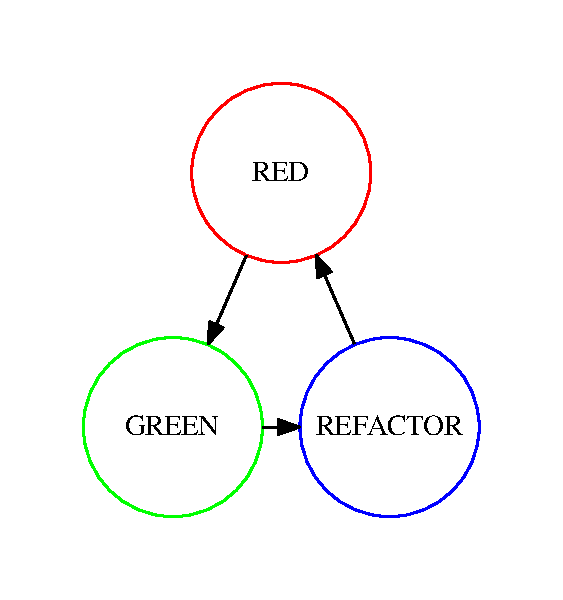
\includegraphics[width=7cm]{img/red-green-refactor.pdf}
}
\only<2-2>{
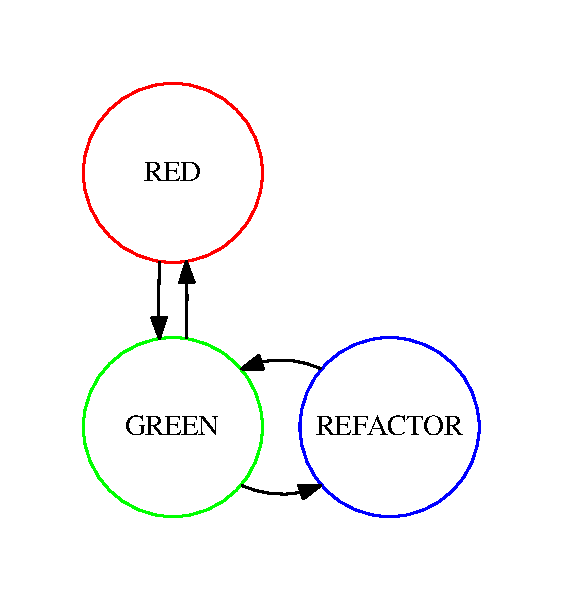
\includegraphics[width=7cm]{img/red-green-refactor-corrected.pdf}
}
\end{center}
\end{frame}

\section{Workshop}

\begin{frame}[fragile]
\frametitle{Workshop}

\begin{enumerate}[<+->]
\item Join channel \texttt{\#refactoring} on Slack\footnote{\url{https://nokiaacademy2016.slack.com}}
\item \texttt{git clone --recurse-submodules <url>\footnote{\url{https://github.com/bodzio528/refactoring-workshop-2016}} <wcopy>}
\item Configure CMake project in QtCreator
\begin{itemize}
	\item GCC or Clang compiler
	\item Debug mode
\end{itemize}
\end{enumerate}
\end{frame}


\subsection{Extract Subroutines}

\begin{frame}
\frametitle{Task \thesubsection: Extract Subroutines}

\begin{narrowblock}{Client's Story}
I want receiving Pause Indication to disable handling of timeout events.
\end{narrowblock}

\pause
\begin{narrowblock}{Hints}
\begin{itemize}[<+->]
\item WET (in fact, massive duplications)
\item Overengineering (try-catch for message dispatch\textellipsis)
\item Split \texttt{receive} method into manageable pieces.
\item New Unit Tests are available on anti-product branch.
\end{itemize}
\end{narrowblock}
\end{frame}

\subsection{Extract Subclasses}

\begin{frame}
\frametitle{Task \thesubsection: Extract Subclasses}

\begin{narrowblock}{Client's Story}
\textbf{BUG!} SnakeController places new food at invalid position! Another FoodReq should be sent in such case.
\end{narrowblock}

\pause
\begin{narrowblock}{Hints}
\begin{itemize}[<+->]
\item This issue is related only to gameboard dimension.
\item SOLID: Single Responsibility.
\item New Unit Tests are available on anti-product branch.
\end{itemize}
\end{narrowblock}
\end{frame}

\subsection{Fight Primitives}

\begin{frame}
\frametitle{Task \thesubsection: Fight Primitives}

\begin{narrowblock}{Client's Story}
Our beloved collegues from Moscow have deployed new, shiny \texttt{Position} and \texttt{Dimension} classes that have some nice features. More important thing -- those are designated as incoming standard of in/out SnakeController communication!
\end{narrowblock}

\pause
\begin{narrowblock}{Hints}
\begin{itemize}[<+->]
\item Scalar values are prone to errors and meaningless on their own. 
\item Expressing programmer thought in domain language is better than obscured bitshift calculations.
\item Mentioned interface update is available on anti-product branch.
\end{itemize}
\end{narrowblock}
\end{frame}

\subsection{Extract Logic}

\begin{frame}
\frametitle{Task \thesubsection: Extract Logic}

\begin{narrowblock}{Client's Story}
I want to receive Score Indication with value of current snake length!
\end{narrowblock}

\pause
\begin{narrowblock}{Hints}
\begin{itemize}[<+->]
\item This is related only to snake internal representation.
\item Tell, do not ask!
\item GRASP: Information Expert.
\item New Unit Tests are available on anti-product branch.
\end{itemize}
\end{narrowblock}
\end{frame}

\subsection{Segregate Interfaces}

\begin{frame}
\frametitle{Task \thesubsection: Extract Interface}

\begin{narrowblock}{Client's Story}
Simon says: Torus World.
\end{narrowblock}

\pause
\begin{narrowblock}{Hints}
\begin{itemize}[<+->]
\item 'T' in config string instead of 'W' indicates this feature enabled.
\item SOLID: Interface Segregation.
\item New Unit Tests are available on anti-product branch.
\end{itemize}
\end{narrowblock}
\end{frame}

\section{Post-Test}
\begin{frame}
\frametitle{Post-Test}
\end{frame}

\begin{frame}
\begin{center}
Thank you for participating!
\end{center}
\end{frame}

\end{document}